\documentclass{article}
\usepackage{tikz}

\setlength{\parindent}{0em}
\setlength{\parskip}{1em}

\author{Garett Lopez}
\date{October 21, 2019}
\title{Sampling Methods Continued}

\begin{document}

\maketitle

\section{Alternative Samplers:}

The key advantage of these methods is that they do not need a good proposal distribution.

\subsection{Affine - Invariant Ensemble Sampler}

Example: emcee -- $``$MCMC Hammer$''$
A general solution; there are no tunable parameters.

The motivation for this method is that we want to be able to handle:

$$ P(\vec{x}) \propto f\left( \frac{-(x_1 - x_2)^2}{2\epsilon} - \frac{(x_1+x_2)^2}{2} \right) $$

for small $\epsilon$


That is:  We want to be able to handle parameters with narrow or curving degeneracies.

The standard M-H method is slow at handling this kind of distribution because a multidimensional Gaussian does not match the degeneracy direction.  One solution, if you know if advance that this will happen, is to change variables to:

$$y_1 = \frac{x_1 - x_2}{\epsilon} \,\,\,\,\,\ y_2 = x_1+x_2$$

But this change can be tedious, because how do you know in advance which change to make?

Affine invariance means it does the same thing irrespective of a variable change of the form:

$$y = \frac{x_i w_i}{\sigma}$$
With $w_i$ being the weights

This affine-invariance method uses an ensemble of walkers, and chooses the next point based on the other walkers positions, with $N_{walkers} \sim 100$. A general tip is to increase the number of walkers.

Walkers start in a ball in the center of the prior volume then wander.

To check convergence, check auto-correlations time and sample until $N_{samp} > 10 t_{auto}$

\tikzset{every picture/.style={line width=0.75pt}} %set default line width to 0.75pt

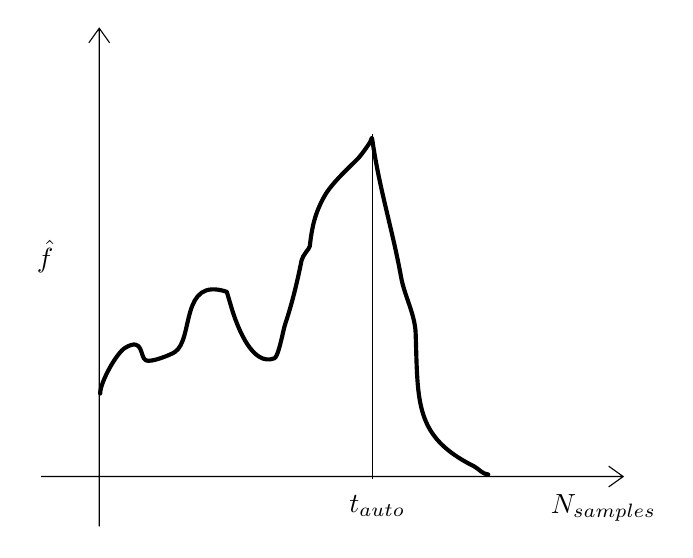
\begin{tikzpicture}[x=0.75pt,y=0.75pt,yscale=-1,xscale=1]
%uncomment if require: \path (0,300); %set diagram left start at 0, and has height of 300

%Shape: Axis 2D [id:dp027594331957089935]
\draw  (50,256) -- (330.5,256)(78.05,40) -- (78.05,280) (323.5,251) -- (330.5,256) -- (323.5,261) (73.05,47) -- (78.05,40) -- (83.05,47)  ;
%Shape: Free Drawing [id:dp9141831406188776]
\draw  [color={rgb, 255:red, 0; green, 0; blue, 0 }  ][line width=1.5] [line join = round][line cap = round] (78.5,216) .. controls (78.5,210.64) and (86.32,196.51) .. (90.5,194) .. controls (99.6,188.54) and (97.46,198.48) .. (100.5,200) .. controls (103,201.25) and (112.6,197.27) .. (114.5,196) .. controls (123.79,189.8) and (116.8,159.43) .. (139.5,167) .. controls (139.53,167.01) and (141.98,175.45) .. (142.5,177) .. controls (144.9,184.19) and (151.91,203.23) .. (162.5,199) .. controls (164.4,198.24) and (166.75,185.24) .. (167.5,183) .. controls (170.95,172.64) and (173.37,162.65) .. (175.5,152) .. controls (176.07,149.13) and (179.36,146.29) .. (179.5,145) .. controls (180.57,135.4) and (182.08,128.96) .. (186.5,121) .. controls (189.97,114.76) and (198.21,107.29) .. (202.5,103) .. controls (204.18,101.32) and (207.18,96.98) .. (208.5,95) .. controls (208.91,94.38) and (209.39,92.26) .. (209.5,93) .. controls (213.03,117.72) and (219.13,135.98) .. (223.5,160) .. controls (225.13,168.96) and (230.2,177.86) .. (230.5,187) .. controls (231.62,220.64) and (229.96,236.73) .. (258.5,251) .. controls (260.9,252.2) and (262.81,255) .. (265.5,255) ;
%Straight Lines [id:da10302871763096366]
\draw    (209.5,91) -- (209.5,257) ;



% Text Node
\draw (153,103) node  [align=left] {};
% Text Node
\draw (52,150) node   {$\hat{f}$};
% Text Node
\draw (321,271) node   {$N_{samples}$};
% Text Node
\draw (212,270) node   {$t_{auto}$};


\end{tikzpicture}


\begin{tabular}{r l}
Pros:  & --There is a simple easy to use python package \\
& --In principle it can be run in parallel (but not in python) \\
& --Preforms well with little tuning.  It works out of the box on small models\\
\end{tabular}

\begin{tabular}{r l}
Cons:  & --It has a well know catastrophic failure mode \\
& --It appears to converge but actually has not \\
& --Happens in higher dimensions (n $\geq$30) \\
& --walkers get stuck at initial positions \\
& --G-R criterion is more robust than the auto-correlation time\\
\end{tabular}

\subsection{Nesting Sampling}

This method basically fits ellipses to the likelihood surface.  It gradually shrinks ellipses to higher peak values.

\begin{tabular}{l l}

Pros: & --Fewer likelihood calculations \\
& --Scales well in higher dimensions \\
& --Computes the Bayesian Evidence \\
 &  \\
Cons: & --Terrible Fortran implementation \\
& --Fragile, requires assumptions about ellipsoid likelihood \\
& --High-overhead (fitting ellipses is expensive in high-D \\

\end{tabular}


This is useful for very slow likelihoods with high dimensions and ellipsoid.  It is reasonable for a very large collaboration (like Plank).

So if we are in high-D and Nesting isn't reliable what do we use?

\subsection{Hamiltonian Monte Carlo}

\underline{Proposal:}  Use local gradients at likelihood evaluations to get a proposal distribution.  The samplers use Hamiltonian Dynamics to explore the space.


\begin{tabular}{l l}

Pros: & --works with up to $10^6$ evaluations \\
& --No free parameters to tune \\
& --Highly parallel \\
 & \\
Cons: & --needs gradient information \\
& --No standard implementation (yet)

\end{tabular}

There is a issue though... How do we get the gradients?

\itemize
\item Analytic Differentiation

Self-explanatory, but requires an analytic likelihood function.

\item Numeric Differentiation

In practice we can use auto-diff.  Effectively, we overload operators to calculate the differentials for that operator and calculate the total differential in the compiler.

\end{document}
